\documentclass[10pt,conference,compsocconf]{IEEEtran}
\usepackage{booktabs}
\usepackage{tabularx}
\usepackage[english]{babel}
\usepackage[ruled]{algorithm}
\usepackage{algpseudocode}
\usepackage{color}
%\let\labelindent\relax
%\usepackage{enumitem}
\let\proof\relax
\let\endproof\relax 
\usepackage{amsthm}
\usepackage[cmex10]{amsmath}
\usepackage{amsfonts}
\usepackage{multicol}
%\let\subcaption\relax
\usepackage[font=small]{subcaption}
\usepackage{graphicx}
\usepackage[hidelinks,bookmarks=false,pdfpagelabels]{hyperref}
\usepackage[nocompress]{cite}
\usepackage{listings}

% definition environment
\newtheorem{definition}{Definition}
\newtheorem{theorem}{Theorem}
\newtheorem{lemma}{Lemma}
\newtheorem{invariant}{Invariant}

% typewriter font family that support hyphenation
%\newcommand\textvtt[1]{{\normalfont\fontfamily{cmvtt}\selectfont #1}}
\hyphenation{MD-List} 
\hyphenation{skip-list}

\algtext*{EndWhile}
\algtext*{EndFor}
\algtext*{EndIf}
\algtext*{EndFunction}
\newcommand\NIL{\text{NIL}}
\newcommand\TRUE{\text{\textbf{true}}}
\newcommand\FALSE{\text{\textbf{false}}}
\newcommand\BREAK{\text{\textbf{break}}}
\newcommand\CONTINUE{\text{\textbf{continue}}}
\newcommand\AND{\;\text{\textbf{and}}\;}
\newcommand\OR{\;\text{\textbf{or}}\;}
\algrenewcommand\algorithmicindent{1em}

\algblockdefx[StructBlock]{Struct}{EndStruct} [1]{\textbf{struct} #1} [0]{}
\algtext*{EndStruct}
\algblockdefx[EnumBlock]{Enum}{EndEnum} [1]{\textbf{enum} #1} [0]{}
\algtext*{EndEnum}
\algblockdefx[ClassBlock]{Class}{EndClass} [1]{\textbf{class} #1} [0]{}
\algtext*{EndClass}
\algblockdefx[MacroBlock]{Define}{EndDefine} [1]{\textbf{define} #1} [0]{}
\algtext*{EndDefine}
\algblockdefx[InlineBlock]{Inline}{EndInline} [2]{\textbf{inline function} \textsc{#1}(#2)} [0]{}
\algtext*{EndInline}
\algblockdefx[SwitchBlock]{Switch}{EndSwitch} [1]{\textbf{switch} (#1)} [0]{}
\algtext*{EndSwitch}

\begin{document}

\title{Lock-free Transactions without Aborts for Linked Data Structures}

\author{\IEEEauthorblockN{Deli~Zhang\hspace{14pt} Damian~Dechev}
    \IEEEauthorblockA{Department of Electrical Engineering and Computer Science\\
        University of Central Florida\\
        Orlando, FL 32817, USA\\
    de-li.zhang@knights.ucf.edu \hspace{14pt} dechev@eecs.ucf.edu}
}

\maketitle

\begin{abstract}
    Non-blocking data structures allow scalable and thread-safe accesses to shared data. 
    They provide individual operations that appear to execute atomically.
    However, it is often desirable to execute multiple operations atomically in a transactional manner.
    This is nearly impossible without revamping the data structures' intricate underlying design.
    In this work, we present a novel technique for implementing high-performance lock-free transactional linked data structures.
    In our approach, transactions insert logically inactive nodes, which are invisible to operations outside the scope of the transaction, into the data structure.
    Through a shared transaction descriptor, it atomically activates all nodes within a transaction upon committing.
    Comparing to generic approaches, such as software transactional memory (STM) and transactional boosting, our approach leverages the semantic knowledge of the data structure implementation to eliminate the overhead of false conflict and operation roll back.
\end{abstract}

%\category{D.1.3}{Concurrent Programming}{Algorithms}
%\terms{Algorithms, Performance}
\begin{IEEEkeywords}
    Concurrent Data Structure, Transactional Memory, Lock-free 
\end{IEEEkeywords}

\section{Introduction}
\label{sec:intro}
With the growing prevalence of multi-core systems numerous highly concurrent non-blocking data structures have emerged~\cite{linden2013skiplist,ellen2010non,braginsky2012lock,zhang2015lockfree,michael2002high}.
Researchers and advanced users have been using libraries like LibCDS~\footnote{http://libcds.sourceforge.net/}, Tervel~\footnote{http://ucf-cs.github.io/Tervel/} and Intel's TBB~\footnote{https://www.threadingbuildingblocks.org/}, which are packed with efficient concurrent implementations of most common data structures.
High level programming languages such as C\#, JAVA and Scala also start to provide concurrent libraries, which allow users who are unaware of the pitfalls of concurrent programming to enjoy the performance benefits safely.
These libraries provide operations that appear to execute atomically when invoked individually.
However, they fall short when users need to execute a sequence of operations atomically (i.e., compose operations in the manner of transaction).
For example, given a linearizable map data structure the following code snippet implementing a simple \texttt{ComputeIfAbsent} pattern~\cite{golan2013concurrent} is error prone.
\begin{lstlisting}[basicstyle=\small,language=JAVA]
    if(!map.containsKey(key)) {
        value = ... // some computation
        map.put(key, value);
    }
\end{lstlisting}
The intention of code is to compute a value and store it in the map, if and only if the map does not already contain the given key.
Despite that, before the invocation of \texttt{put} and after the execution of \texttt{containsKey} another thread may have stored a value associated with the same key.
That value will get overwritten once the current thread finishes the \texttt{put} operation. 
Many Java programs encounter bugs that are caused by such non-atomic composition of operations~\cite{shacham2011testing}.
This sometimes force users to fall back to coarse-grained locks, which annihilates concurrency.

The problem of implementing high-performance transactional data structures~\footnote{Also referred as \emph{atomic composite operations}~\cite{golan2013concurrent}} is thus an important one and has gained much attention recently~\cite{golan2013concurrent,bronson2010transactional,herlihy2008transactional,gramoli2013composing,golan2015automatic,hassan2014integrating,koskinen2010coarse}. 
In this paper, we refer to a sequence of atomic operations as a transaction.
We consider a concurrent data structure `transactional' if it executes transactions 1) atomically (i.e., if one operation fails the entire transaction should abort), and 2) in isolation (i.e., concurrent executions of transactions appears to take effect in some sequential order).
%Supporting transactional operations in concurrent sets~\cite{bronson2011composable} are especially rewarding, because they are the fundamental building blocks of in-memory databases~\cite{}.
General purpose software transactional memory (STM)~\cite{shavit1997software,herlihy2003software} can be used to easily construct transactional data structures from their sequential counterparts: any operations executed within an STM transaction are guaranteed to be transactional.
Despite the appeal of straightforward implementation, this approach has not gain practical acceptance due to significant runtime overhead~\cite{cascaval2008software}.
An STM instruments threads' memory accesses, which records the locations a thread read in a \emph{read set}, and the locations it wrote in a \emph{write set}. 
conflicts are detected among the \emph{read/write sets} of different threads. 
In the presence of conflicts, only one transaction is allowed to commit while the others are aborted and restarted.
Apart from the overhead of memory instrumentation, excessive transaction aborts in the presence of data structure "hot-spot" (memory locations that are constantly accessed by threads, e.g., the head node of a linked list) limit the overall concurrency~\cite{herlihy2008transactional}.
\begin{figure}[h]
    \centering
    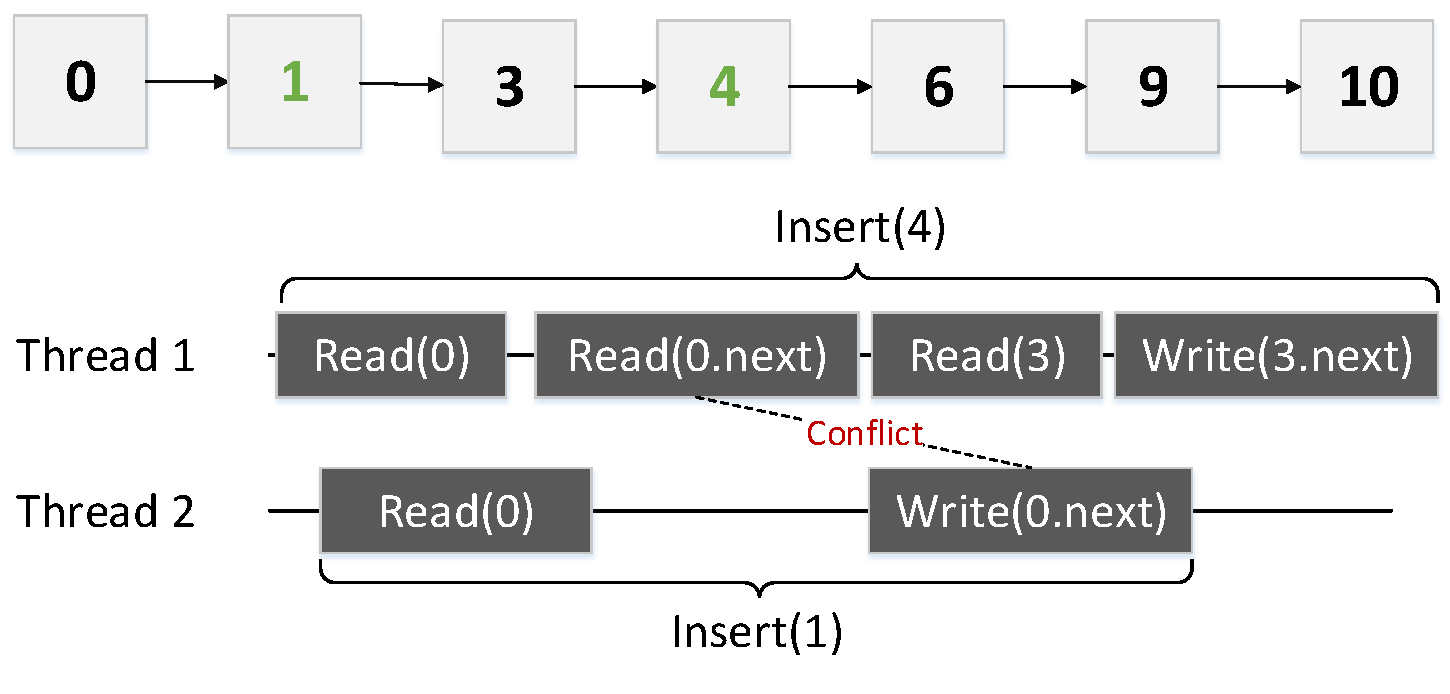
\includegraphics[width=0.8\columnwidth]{figure/stmconflict.pdf}
    \caption{False Conflict in STM}
    \label{fig:stmconflict}
\end{figure}
Figure~\ref{fig:stmconflict} illustrate such an example.
It shows a set implemented as an ordered linked list, where each node has two fields, an integer value and a pointer to the next node.
The initial state of the set is $\{0,3,6,9,10\}$.
Thread 1 and thread 2 intend to insert 4 and 1 respectively.
Since these two operations commute, there is no reason why they cannot be executed concurrently~\cite{clements2015scalable}.
In fact, concurrent linked list implementations employing lock-free~\cite{michael2002high} or fine-grained locking synchronizations~\cite{bayer1977concurrency} do allow concurrent execution of the two operations.
Nevertheless, these operations have a read/write conflict and the STM has to abort one of them. 
The inherent disadvantage of STM concurrency control is that low-level memory access conflicts do not necessarily correspond to high-level semantic conflicts.
%Some efforts have be done to alleviate the situation by somehow inferring part of the semantic either through user annotation or.

Transactional boosting~\cite{herlihy2008transactional} is a methodology for transforming linearizable concurrent data structures into transactional data structures.
The basic idea behind boosting is intuitive: if two operations commute they are allowed to proceed without interference (i.e., synchronization happens on operation level); otherwise they need to be synchronized on the transaction level.
It treats the original data structure as black box and uses \emph{abstract lock} to ensure that non-commutative method calls never occur concurrently. 
For each operation in a transaction, the boosted data structure calls corresponding method of the underlying linearizable data structure after acquiring the abstract lock associate with that call. 
A transaction abort when it fails to acquire an abstract lock, and it recovers from failure by invoking the inverses of already executed calls. 
This approach eliminates the excessive aborts associated with STM-based transactional data structures, but it still suffer from performance penalty of rolling back partially executed transactions.
Moreover, since it relies on locks for transactional level synchronization, the progress guarantee of the boosted data structures is effectively degraded if the original linearizable data structures are non-blocking.
%\begin{figure}[h]
    %\centering
    %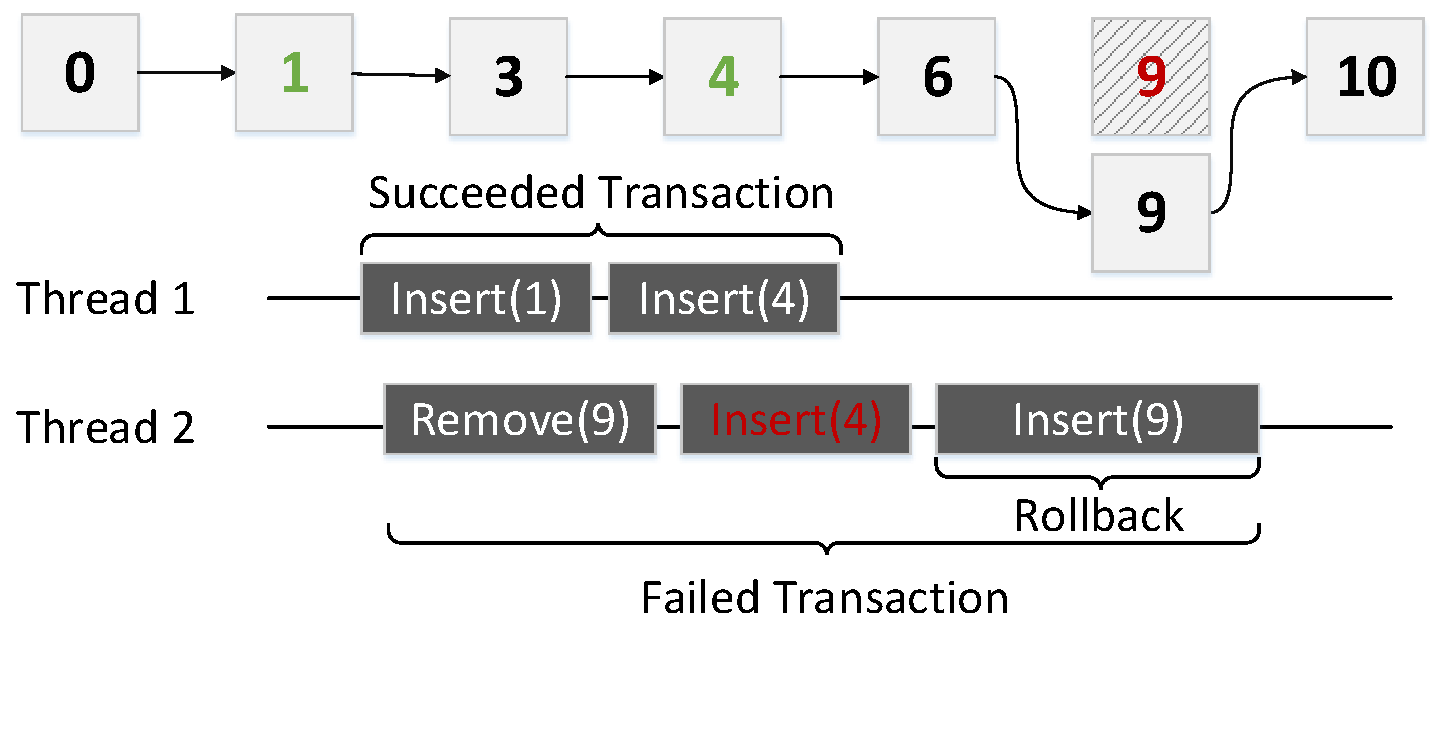
\includegraphics[width=0.9\columnwidth]{figure/boosting.pdf}
    %\caption{Rollbacks in Transactional Boosting}
    %\label{fig:boosting}
%\end{figure}
%In the boosted linked list shown in Figure~\ref{fig:boosting}, the abstract lock is pertaining to each key.  
%thread 1 tries to execute \texttt{Insert(1)} and \texttt{Insert(4)} in a transaction while thread 2 tries to execute \texttt{Remove(9)} and \texttt{Insert(4)} transactionally.
 
In this paper, we present an implementation technique to enable support of lock-free transactions for linked data structures using only single word \texttt{ComapreAndSwap} synchronization primitive.
By a linked data structure we mean one that comprises a set of of data nodes organized by references. 
Each node has one inbound reference and can have one (e.g., linked list), two (e.g., binary tree), or more (e.g., B-tree and multi-dimensional linked list) out bound references.
Consider the three basic write operations one can perform on a node: insertion, deletion, and update.
In existing data structure implementations, these operations act directly on different fields of a physical node, and the results are rendered immediately in the state of the abstract data type (ADT).
This proves to be a problem for transaction isolation, which requires the effect of an operation to be invisible to operations outside the transaction scope before the transaction commits.
In our transactional data structure implementations, we design an indirect procedure to update or delete nodes by inserting new nodes that replace exiting nodes in the data structure.
We also associate a logical status with each node by embedding \emph{transaction descriptors} in them.
A descriptor is shared among all the nodes within the same transaction, and it stores the operation context as well as a flag indicating whether the transaction has committed.
A node's logical status is determined by the type of operation and the status of the transaction.
For example, a physical node with a descriptor indicating transaction failure and the fact that its been inserted by a deletion operation actually implies the logical existence of the node.
As a result, the state of the ADT is determined by the interpreting the logical status of all nodes.
Our approach has the following algorithmic characteristics that aim to provide the same level concurrency as the state-of-the-art lock-free data structures.
\begin{itemize}
    \item In-progress and failed transactions do not alter the state of abstract date types
    \item Transactions do not abort upon node access conflict; instead they help delayed operations to achieve lock-freedom
    \item Rolling back executed operations in failed transactions is not necessary as the nodes will remain logically inactive
\end{itemize}

In our experimental evaluation, we compare transactional linked list and binary search trees built using RSTM, transactional boosting, and out approach on a 64-core NUMA and a 12-core SMP system for three types of workload. 
%The result shows that on the NUMA system our algorithm outperforms the alternative approaches by an average of $50\%$ under high concurrency.
%On the SMP system, our algorithm achieves the same level of performance as the best skiplist-based approach for mixed workload and outperforms the alternatives for insert-only workload. 

The rest of the paper is organized as follows. 
In Section~\ref{sec:related}, we review existing approach on constructing transactional data structures.
In Section~\ref{sec:algorithm}, we explain our algorithms in details.
We present the transactional linked list and binary search tree in Section~\ref{sec:application}.
We reason about its correctness and progress properties in Section~\ref{sec:correctness}.
The performance evaluation and result analysis is given in Section~\ref{sec:experiment}.
We conclude the paper in Section~\ref{sec:conclusion}.

\section{Related Work}
\label{sec:related}
%1: lock-free data structures with thread-level synchronization techniques
%2: transaction synchronization
A transactional execution of data structure operations can be seen as a restricted form of \emph{software transactions}~\cite{harris2010transactional}.
%The scope of the data and the are well defined according to the semantics of the data structure.
%This opens up opportunity for enabling data structure specific optimizations. 
%The users of concurrent data structures have to devise their own concurrency control scheme. 
Straightforward generic constructions can be implemented by executing all the shared memory accesses in \emph{atomic sections}, which can employ either optimistic (e.g., STM) or pessimistic (e.g., lock inference) concurrency control.
More sophisticated approaches~\cite{bronson2010transactional,herlihy2008transactional,golan2015automatic} exploit semantic conflict detection for transaction level synchronization to reduce benign conflicts.
In our work, we marry the benefit of fine-grained thread level synchronization with semantic conflict detection to implement transactional linked data structures without the overhead of atomic section synchronizations.

\subsection{Transactional Memory}
Initially proposed as a set of hardware extensions by Herlihy and Moss~\cite{herlihy1993transactional}, transactional memory was intended to facilitate the development of lock-free data structures.
%Even with Intel's recent release of commercial support of best-effort hardware transaction memory (HTM) in their Haswell processors, 
However, due to current HTM's cache-coherency based conflict detection mechanism, transactions are subject to spurious failures during page faults and context switches~\cite{dice2009early}.
This along with excessive aborts under moderate contention~\cite{christina2015resource} make HTM less desirable for implementing transactions in non-blocking data structures.
Thus, considerable amount of work and ingenuity has instead gone into designing lock-free data structures using low-level synchronization primitives such as \texttt{CompareAndSwap}, which empowers researchers to devise algorithm-specific fine-grained concurrency control schemes.

The first software implementation of transactional memory was proposed by Shavit and Touitou~\cite{shavit1997software}, which only supports a static set of data items.
Over the years, improvements have been achieved in terms of functionality~\cite{herlihy2003software}, consistency properties~\cite{guerraoui2008correctness}, progress guarantees~\cite{marathe2006lowering}, and performance~\cite{saha2006mcrt,dice2006transactional}. 
Despite heavy research investment, there is an increasing realization that the read/write conflicts inherently provide insufficient support for concurrency when shared objects are subject to contention~\cite{koskinen2010coarse}.
Meanwhile as design choices have been exhaustedly explored~\cite{marathe2004qualitative,marathe2004design}, other limitations faced by STM with regard to usability~\cite{Rossbach2010transactional}, performance~\cite{cascaval2008software}, and expressiveness~\cite{guerraoui2008obstruction} also began to surface.
It has been suggested that STM may not deliver the promised efficiency and simplicity for every scenario, and multitude of approaches should be explored catering to different needs~\cite{attiya2010inherent}.
%Unlike STM-based data structures, our approach eliminate the need to abort transactions.

\subsection{Lock Inference}
The above mentioned STM implementations are typically \emph{optimistic}, which means they execute under the assumption that interferences are unlikely to occur.
They also maintain expensive undo-logs to allow rollback in case a transaction do experience interference.
In light of this shortcoming, pessimistic alternatives based on lock inference has been proposed~\cite{mccloskey2006autolocker}.
These algorithms synthesize enough locks through static analysis to prevent data races in atomic sections.
The choice of locking granularity will have an impact on the trade-off between concurrency and overhead.
Some approaches require programmers' annotation~\cite{golan2013concurrent} to specify the granularity, others automatically infer locks at a fixed granularity~\cite{emmi2007lock} or even multiple granularities~\cite{cherem2008inferring}.
Nevertheless, most work associate locks with memory locations, which may lead to reduced parallelism due to false conflict as seen in STM. 
Applying these approaches to real-world programs also faces scalability changes in the presence of large libraries ~\cite{gudka2012lock} because of the high cyclomatic complexity~\footnote{A measure of the number of linearly independent execution paths~\cite{mccabe1976complexity}.} involved in the static analysis process.
Moreover, the use of locks degrades any non-blocking progress guarantee one might expected from using a non-blocking library.
%Kempf2014combining combines lock inference and stm.

\subsection{Semantic Conflict Detection}
Considering the imprecise nature of data-base conflict detection, semantic-based approaches has been proposed to identify conflicts at high-level (e.g., two commutative operations would not raise conflict even though they may access and modify the same data) which enables greater parallelism.
Because semantically independent transactions may have structural conflicts, some other concurrency control mechanism must be used to protect accesses to the underlying data structure.
This results in a two-layer concurrency control.
Transactional boosting proposed by Herlihy~\cite{herlihy2008transactional} was the first dedicated treatment on building highly concurrent transactional data structures using a semantic layer of abstract locks. 
Transactional boosting is pessimistic in that it acquires locks eagerly before the method calls, but it still requires operation rollback because not all locks are acquires at once.
%PTB, black box design, forfiet data structure specific optimization, need to reverse operation upon failure
Koskinen et al.~\cite{koskinen2010coarse} later generalize this work and introduce a formal framework called coarse-grained transactions.
Hassan et al.~\cite{hassan2014developing} proposed an optimistic version of boosting, which employs an white box design and provide some performance benefits.
Other STM variants, such open nested transactions~\cite{ni2007open} supports a more relaxed transaction model that leverages some semantic knowledge based on programmer's input.
The relaxation of STM systems and its implication on composability has been studied by Gramoli et al.~\cite{gramoli2013composing}.
The work by Golan-Gueta et al.~\cite{golan2015automatic} apply commutativity specification obtained from programmers input to inferring locks for abstract data types.
All these approaches require the underlying data structure to be linearizable.
%Our approach, do not track read/write set, highly concurrent, Optimistic lock-free
%we leverage the semantic knowledge of the data structure implementation, 

\section{Algorithm}
\label{sec:algorithm}
Non-blocking algorithms for linked data structures have been extensively studied because their distribute memory layout provides access parallelism and good scalability under high levels of contention~\cite{linden2013skiplist,zhang2015lockfree,michael2002high}.
To the best of our knowledge, there is no non-blocking linked data structure that provides native support for transactions.
To ensure atomicity in non-blocking transaction execution without an additional layer of synchronization, a write operation needs to either ``hide'' its effect until the transaction commits or revert its modifications upon transaction failure.
We follow the former strategy because the latter requires extra coordinations between operations in different transaction in order to achieve isolation.
To effectively ``hide'' the newly inserted nodes before transaction completes, we embed a transaction-status-dependent logical flag in them. 
This is similar to the \emph{logical deletion} technique, which is used in~\cite{harris2001pragmatic} to ensure list integrity and in~\cite{linden2013skiplist,zhang2015lockfree} to speedup the deletion process.
Logical deletion encodes a binary logical status in a node's bit-marked next pointer, whereas our approach embeds a multi-value transaction status in the descriptor object shared among nodes.
The key challenge remains to design a deletion and update process that allow logically invisible modification.
We achieve this goal by having them insert physical nodes that are logically inactive instead of modify the data structure directly.
In this section we explain the basic data structures as well as two core procedures that are shared among different kinds of linked data structures.

\subsection{Data Structure}
We define the generic node structure used in the rest of the paper in Algorithm~\ref{alg:nodestructure}. 
A node contains a key-value pair, and an array of child pointers $child[N]$, where $N$ depends on the concrete data type (e.g., 1 for linked lists, 2 for binary trees, etc.)
It also stores a reference to the shared transaction descriptor object $desc$ and an index $opid$ that provide reference to the operation pertaining to this node (i.e., $desc.ops[opid]$ is the operation that inserted this physical node).
Finally, it has a reference $repl$ to the node it replaces (if it replaces anything).
The descriptor object~\cite{herlihy2012art} \textsc{Desc} is a data structure used in lock-free programming to announce steps that cannot be done by a single atomic instruction.
The functionalities of a transactional descriptor are two folds: 1) it stores all the necessary context for any thread to finish a pending transaction; and 2) it provides the transaction status shared among all nodes participated in the same transaction.
Each operation structure keeps a key-value pair for the operation and an enumeration of operation type, the value of which depends on the concrete data types.

\begin{algorithm}[h]
    \caption{Node Structures}
    \label{alg:nodestructure}
    \vspace{-0.2in}
    \begin{multicols}{2}
        \begin{algorithmic}[1]
            \Enum{Status}
            \State \textbf{InProgress}
            \State \textbf{Succeeded}
            \State \textbf{Failed}
            \EndEnum
            \Struct{Desc}
            \State \textbf{int} $size$
            \State \textbf{Stauts} $flag$
            \State \textbf{Operation} $ops[\;]$
            \EndStruct
            \Struct{Operation}
            \State \textbf{int} $type,key$
            \State \textbf{void*} $val$
            \EndStruct
            \Struct{Node}
            \State \textbf{int} $key,opid$
            \State \textbf{void*} $val$
            \State \textbf{Node*} $child[N],repl$
            \State \textbf{Desc*} $desc$
            \EndStruct
            \end{algorithmic}
    \end{multicols}
    \vspace{-0.15in}
\end{algorithm}

\begin{algorithm}[h]
    \caption{Pointer Marking}
    \label{alg:pointermarking}
    \begin{algorithmic}[1]
        \State \textbf{const int} $F_{adp} \gets \texttt{0x1}$
        \Define{SetMark}{$p,\;m$} $(p\;|\;m)$
        \EndDefine
        \Define{ClearMark}{$p,\;m$} $(p\;\&\;\sim m)$
        \EndDefine
        \Define{IsMarked}{$p,\;m$} $(p\;\&\;m)$
        \EndDefine
    \end{algorithmic}
\end{algorithm}

We employ the pointer marking technique described by Harris~\cite{harris2001pragmatic} to mark adopted child nodes as well as logically deleted nodes. 
The macros for pointer marking are defined in Algorithm~\ref{alg:pointermarking}.
The $F_{adp}$ flag is co-located with the $child$ pointers.

\subsection{Lock-free Node Replacement}
\label{sec:noderepl}
All write operations in our approach try to insert new physical nodes.
If no physical node with the same key exists, lock-free insertion can be done by simply swing the next pointer of the predecessor node~\cite{zhang2015lockfree,harris2001pragmatic}, but more often, nodes are inserted to replace an existing physical node in order to change its logical status.
For example, to delete the exiting node 4 from a linked list as shown in Figure~\ref{fig:nodedeletion} we insert a new node marked for logical deletion in place of the original node.
\begin{figure}[h]
    \centering
    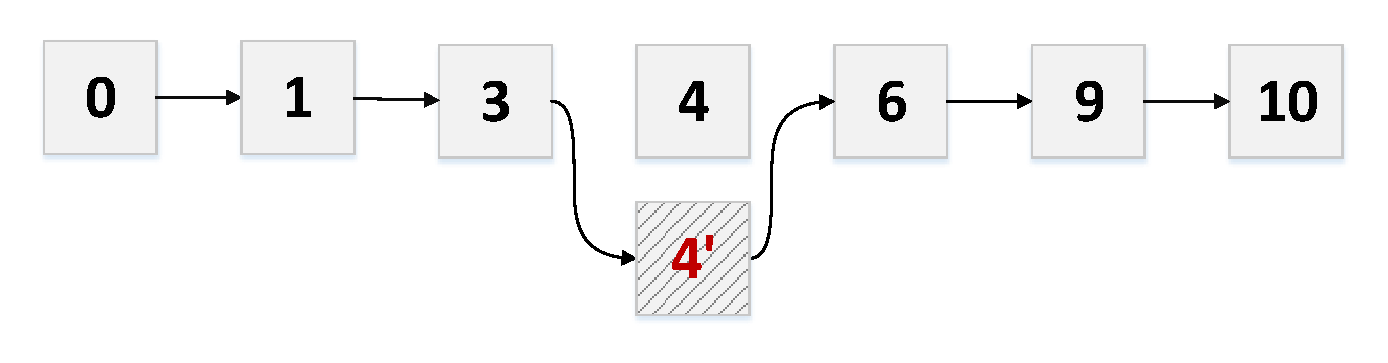
\includegraphics[width=0.8\columnwidth]{figure/deletion.pdf}
    \caption{Node Deletion}
    \label{fig:nodedeletion}
\end{figure}

\begin{algorithm}[h]
    \caption{Node Replace}
    \label{alg:replace}
    \begin{algorithmic}[1]
        \Function{Replace}{$\textbf{Node*}\;pred,\;\textbf{Node*}\;repl\;\textbf{Node*}\;n$}
        \State $n.adopt \gets repl$
        \If {$\text{\textsc{CAS}}(\&pred.child[i],\;repl,\;n)$} \label{l:link}
        \State \Call{AdoptChild}{$n$} \label{l:adoptself}
        \State \Return \TRUE
        \Else
        \State \Return \FALSE
        \EndIf
        \EndFunction
        \Statex
        \Function{AdoptChild}{$\textbf{Node*}\;n$}
        %\If {$n = \NIL$}
        %\State \Return
        %\EndIf
        \State \textbf{Node*} $repl \gets node.repl$
        \If {$repl=\NIL$}
        \State \Return
        \EndIf
        \State \textbf{Node*} $child$ 
        \For {$i \in [0, N)$} \label{l:adoptionfor}
        \State $child \gets \textsc{FetchAndOr}(\&repl.child[i],\;F_{adp})$ \label{l:setadp} 
        \State $child \gets \textsc{ClearMark}(child,\;F_{adp})$
        \State $\text{\textsc{CAS}}(\&n.child[i],\;\NIL,\;child)$ \label{l:adopt}
        \EndFor
        \State $n.repl \gets \NIL$
        \EndFunction
        \end{algorithmic}
\end{algorithm}

This requires the child nodes of node being replaced to be transfered to the new node in a lock-free manner.
The \textsc{Replace} function inserts a new node $n$ to replace the $i$th child $repl$ of its predecessor $pred$.
We link $pred.child[i]$ to the new node on line~\algref{alg:replace}{l:link}, and proceed to adopt child nodes from $repl$ in the helper function \textsc{AdoptChild}.
Before a child pointer can be copied, we must safeguard it so that it cannot be changed by concurrent insertions while the copy is in progress.
This is done by setting the $F_{adp}$ flag in the child pointers (line~\algref{alg:replace}{l:setadp}).
Once the flag is set either by this thread or by other threads, the function proceeds to copy the pointer to $n$ (line~\algref{alg:replace}{l:adopt}). 
Finally, the descriptor field in $n$ is cleared to designate the operation's completion.

\subsection{Transaction Execution}
\label{sec:txnexec}
%The caveat is that the read operations need to check a node's status to ensure it is in a consistent status or even help the write operation to finish the remaining steps.
In our approach, we treat nodes as the natural units for conflict detection.
%; e.g., insert 3 modifies node 2, but update 3 modifies node 3
Write operations inserting nodes with different keys are allowed to execute concurrently.
Should conflicts among write operations occur, threads help finish the delayed transaction starting from the node in conflict.
The \textsc{ExecuteOps} function in Algorithm~\ref{alg:transaction} execute operations starting from $opid$ in the transaction descriptor $desc$.
The thread initiating the transaction will start from $opid=0$, while other thread might concurrently invoke this method to help unfinished operations with $opid\in[1,desc.size)$.
The method consists of a while loop (line~\algref{alg:transaction}{l:txnwhile}) that executes each operation in order.
The next operation will only be executed if the previous operation completes successfully.
Otherwise, it indicates some unsatisfied precondition and the transaction aborts. 
The concrete \textsc{ExecuteOp} function varies slightly among different data types.
We explain them in details in Section~\ref{sec:application}.
Once all operations completes successfully we atomically update the transaction status with a succeeded flag (line~\algref{alg:transaction}{l:txnsuccess}).

\begin{algorithm}[h]
    \caption{Transaction Execution}
    \label{alg:transaction}
    \begin{algorithmic}[1]
        \Function{ExecuteOps}{$\textbf{Desc*}\;desc,\;\textbf{int}\;opid$}
        \State $ret \gets \TRUE$
        \While {$desc.flag = InProgress$ $\AND ret \AND$ $opid < desc.size$} \label{l:txnwhile}
        \State $\textbf{Operation*} op \gets \&desc.ops[opid]$
        \State $ret \gets \Call{ExecuteOp}{op}$
        \State $opid \gets opid + 1$
        \EndWhile
        \If {$ret = \TRUE$}
        \State $\text{\textsc{CAS}}(\&desc.flag,\;InProgress,\;Succeeded)$ \label{l:txnsuccess}
        \Else
        \State $\text{\textsc{CAS}}(\&desc.flag,\;InProgress,\;Failed)$        
        \EndIf
        \EndFunction
        \end{algorithmic}
\end{algorithm}



\section{Application Examples}
\label{sec:application}
\_

\subsection{Linked List}
\_

\subsection{Binary Search Tree}
\_

\section{Correctness}
\label{sec:correctness}
\_

\section{Experimental Results}
\label{sec:experiment}
\_

\section{Conclusion}
\label{sec:conclusion}
\_


\bibliographystyle{IEEEtran}
\bibliography{citation}

\end{document}
